\documentclass{report}
\usepackage[utf8]{inputenc}
\usepackage{hyperref}
\usepackage[english]{babel}
\usepackage{graphicx}
\graphicspath{ {./} }

\title{Assignment 1 - Data Mining}
\author{Kuldeep kumar solanki}
\date{25th September 2020}

\begin{document}

\makeatletter
    \begin{titlepage}
        \begin{center}
            
\includegraphics[width=0.7\linewidth]{images/redlogo.jpg}\\[4ex]
            {\huge \bfseries  \@title }\\[2ex] 
            {\LARGE  \@author}\\[50ex] 
            {\large \@date}
        \end{center}
    \end{titlepage}
\makeatother
\thispagestyle{empty}
\newpage

\tableofcontents
\newpage

\section{Assignment Objective}
\justify The assignment aims to show the impact of \href{https://www.covid19india.org/}{\underline{COVID-19}} in India between date 15th March 2019 to 5th September 2019. It uses input data from \href{https://api.covid19india.org/}{\underline{COVID-19 API}} portal.
\subsection{Assumptions}
\justify There are some states in India whose district data is not clearly available in the API(csv file). So i merged the districts of these states into one district and give this district name of the state.
I merged Delhi, Assam, Goa, Telangana. Along with this i also merged the 3 district into one district and call it Mumbai.
\subsection{Assumptions Effects}
\justify As there are many districts in Assam and Telangana, so when we merge these smaller districts into one district there will be effect of these in the neighbor mean, state mean, state Z-Score and in neighbor Z-Score. Also we are not able to find the hotspot and coldspot of these states.
\newpage

\section{Graphs}
\subsection{Understanding GRAPHS}
\justify Each graphs provided in this section aims to show that the y-axis is the metric(like mean, overall cases, z-score) and x axis is the district which I are considering. With help of these graphs the comparison between district is made.
\newline
Each district is associated with a unique ID starting from 101. X-axis in each graph shows the district id associated with the district.
\newline 
The Y-axis values in each graph is calculated in the time span of 15th March to 5th September.

\subsection{Overall Cases GRAPH}
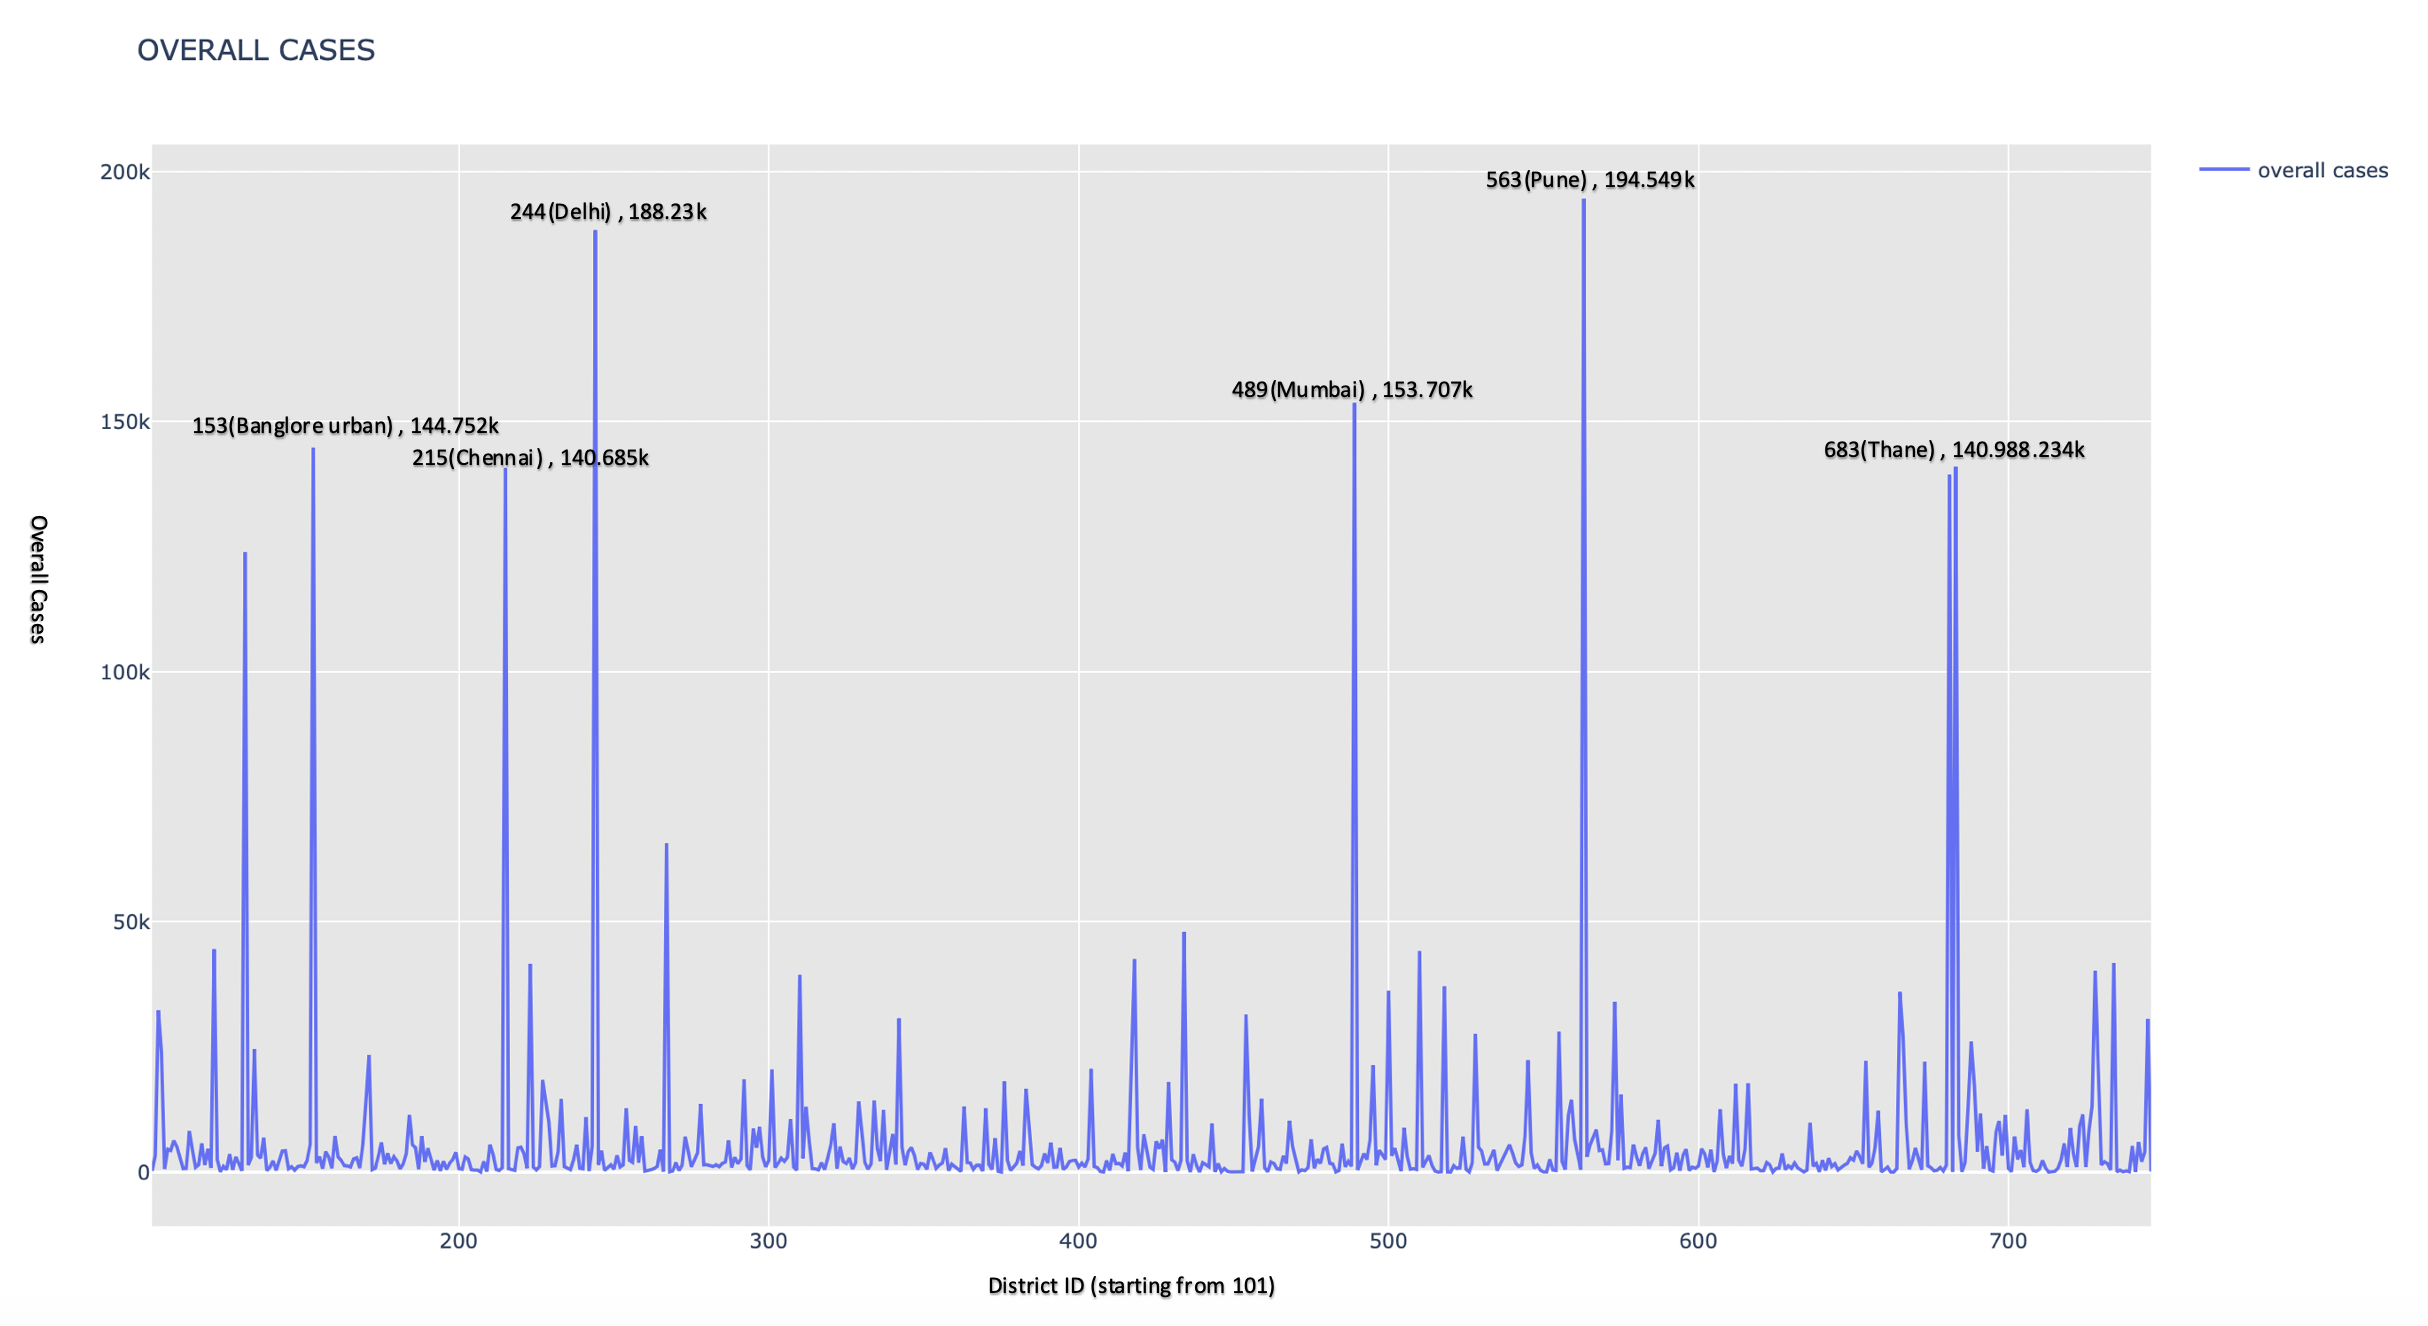
\includegraphics[scale=0.32]{images/OverallCases.png}
\centerline{\textbf{Figure 1}} \newline\newline
\justify \textbf{Figure 1} aim to show the impact of COVID-19 cases in India with respect to every district. The X-axis shows the district ID which is associated with the district name. The Y-axis shows the total number of cases. 
\newline \textbf{Banglore urban, Pune, Mumbai, Chennai, Thane} shows the very high impact of COVID-19. On an average it is above 1.5 Lakh which is very huge for district. 
    
\newpage
\subsection{Neighbor Mean GRAPH}
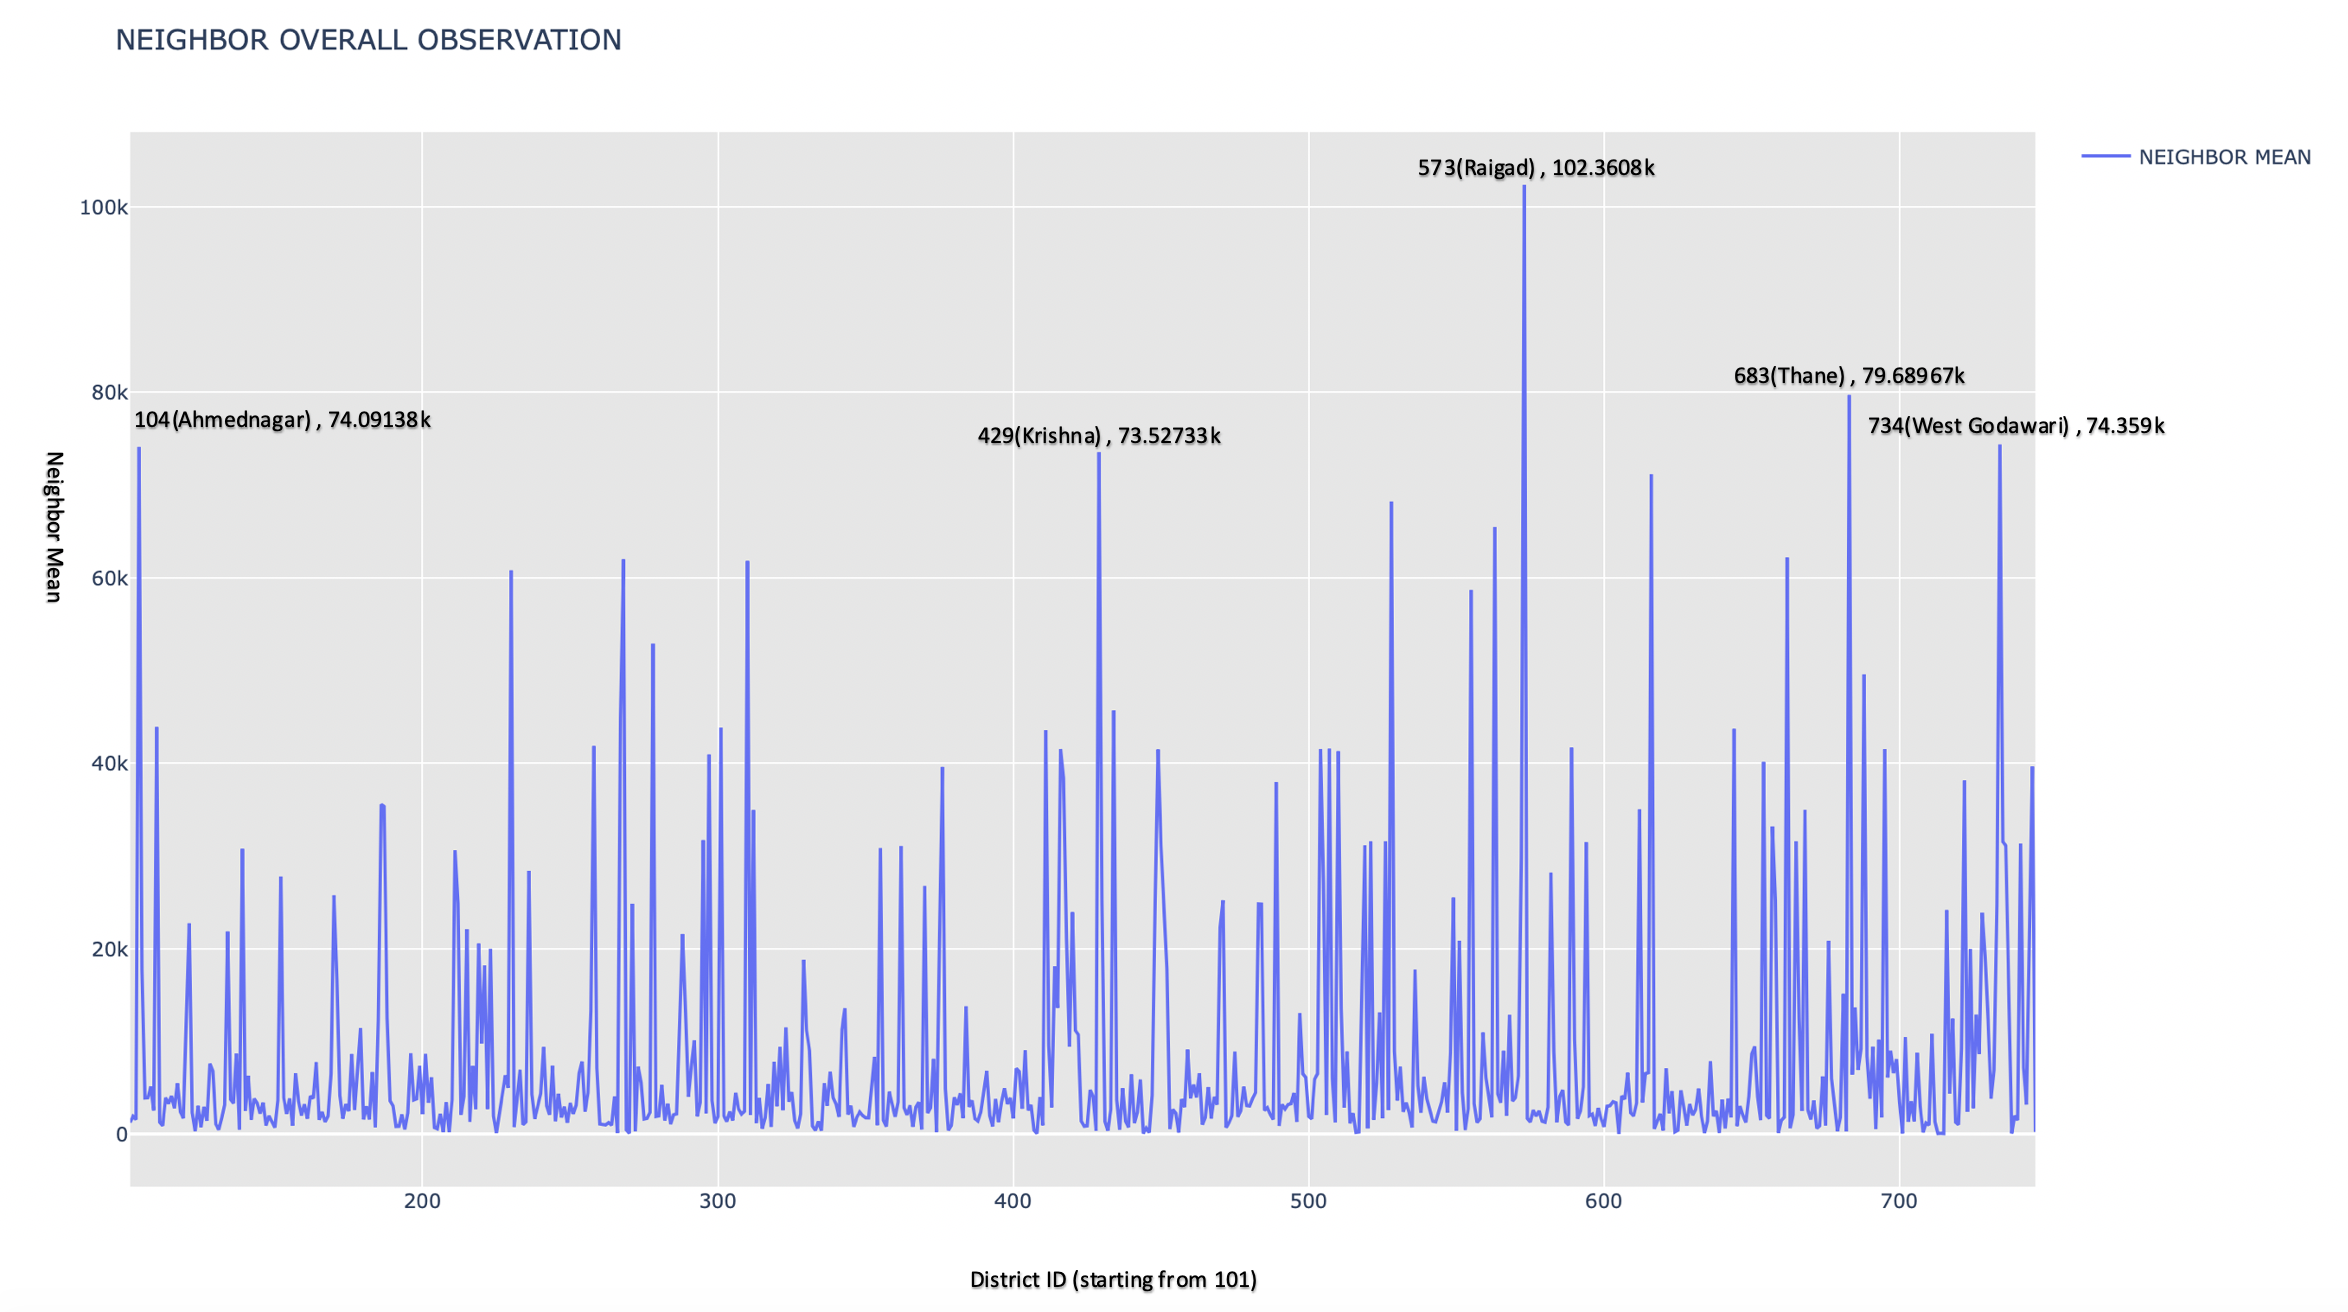
\includegraphics[scale=0.335]{images/Neighbor Mean.png}
\centerline{\textbf{Figure 2}} \newline\newline
\justify \textbf{Figure 2} aim to show the impact of COVID-19 on a particular district with respect to its neighborhood district COVID-19 cases. The Y-axis shows the average(mean) value of the number of cases in neighbourhood districts. The X-axis shows which district we are considering when we are taking average of number of cases in neighbourhood districts. 
\newline \textbf{Raigad, Thane, Ahmednagar, Krishna, West Godawari} are the top 5 districts which are badly affected by its neighbour district.

\newpage    
\subsection{State Mean GRAPH}
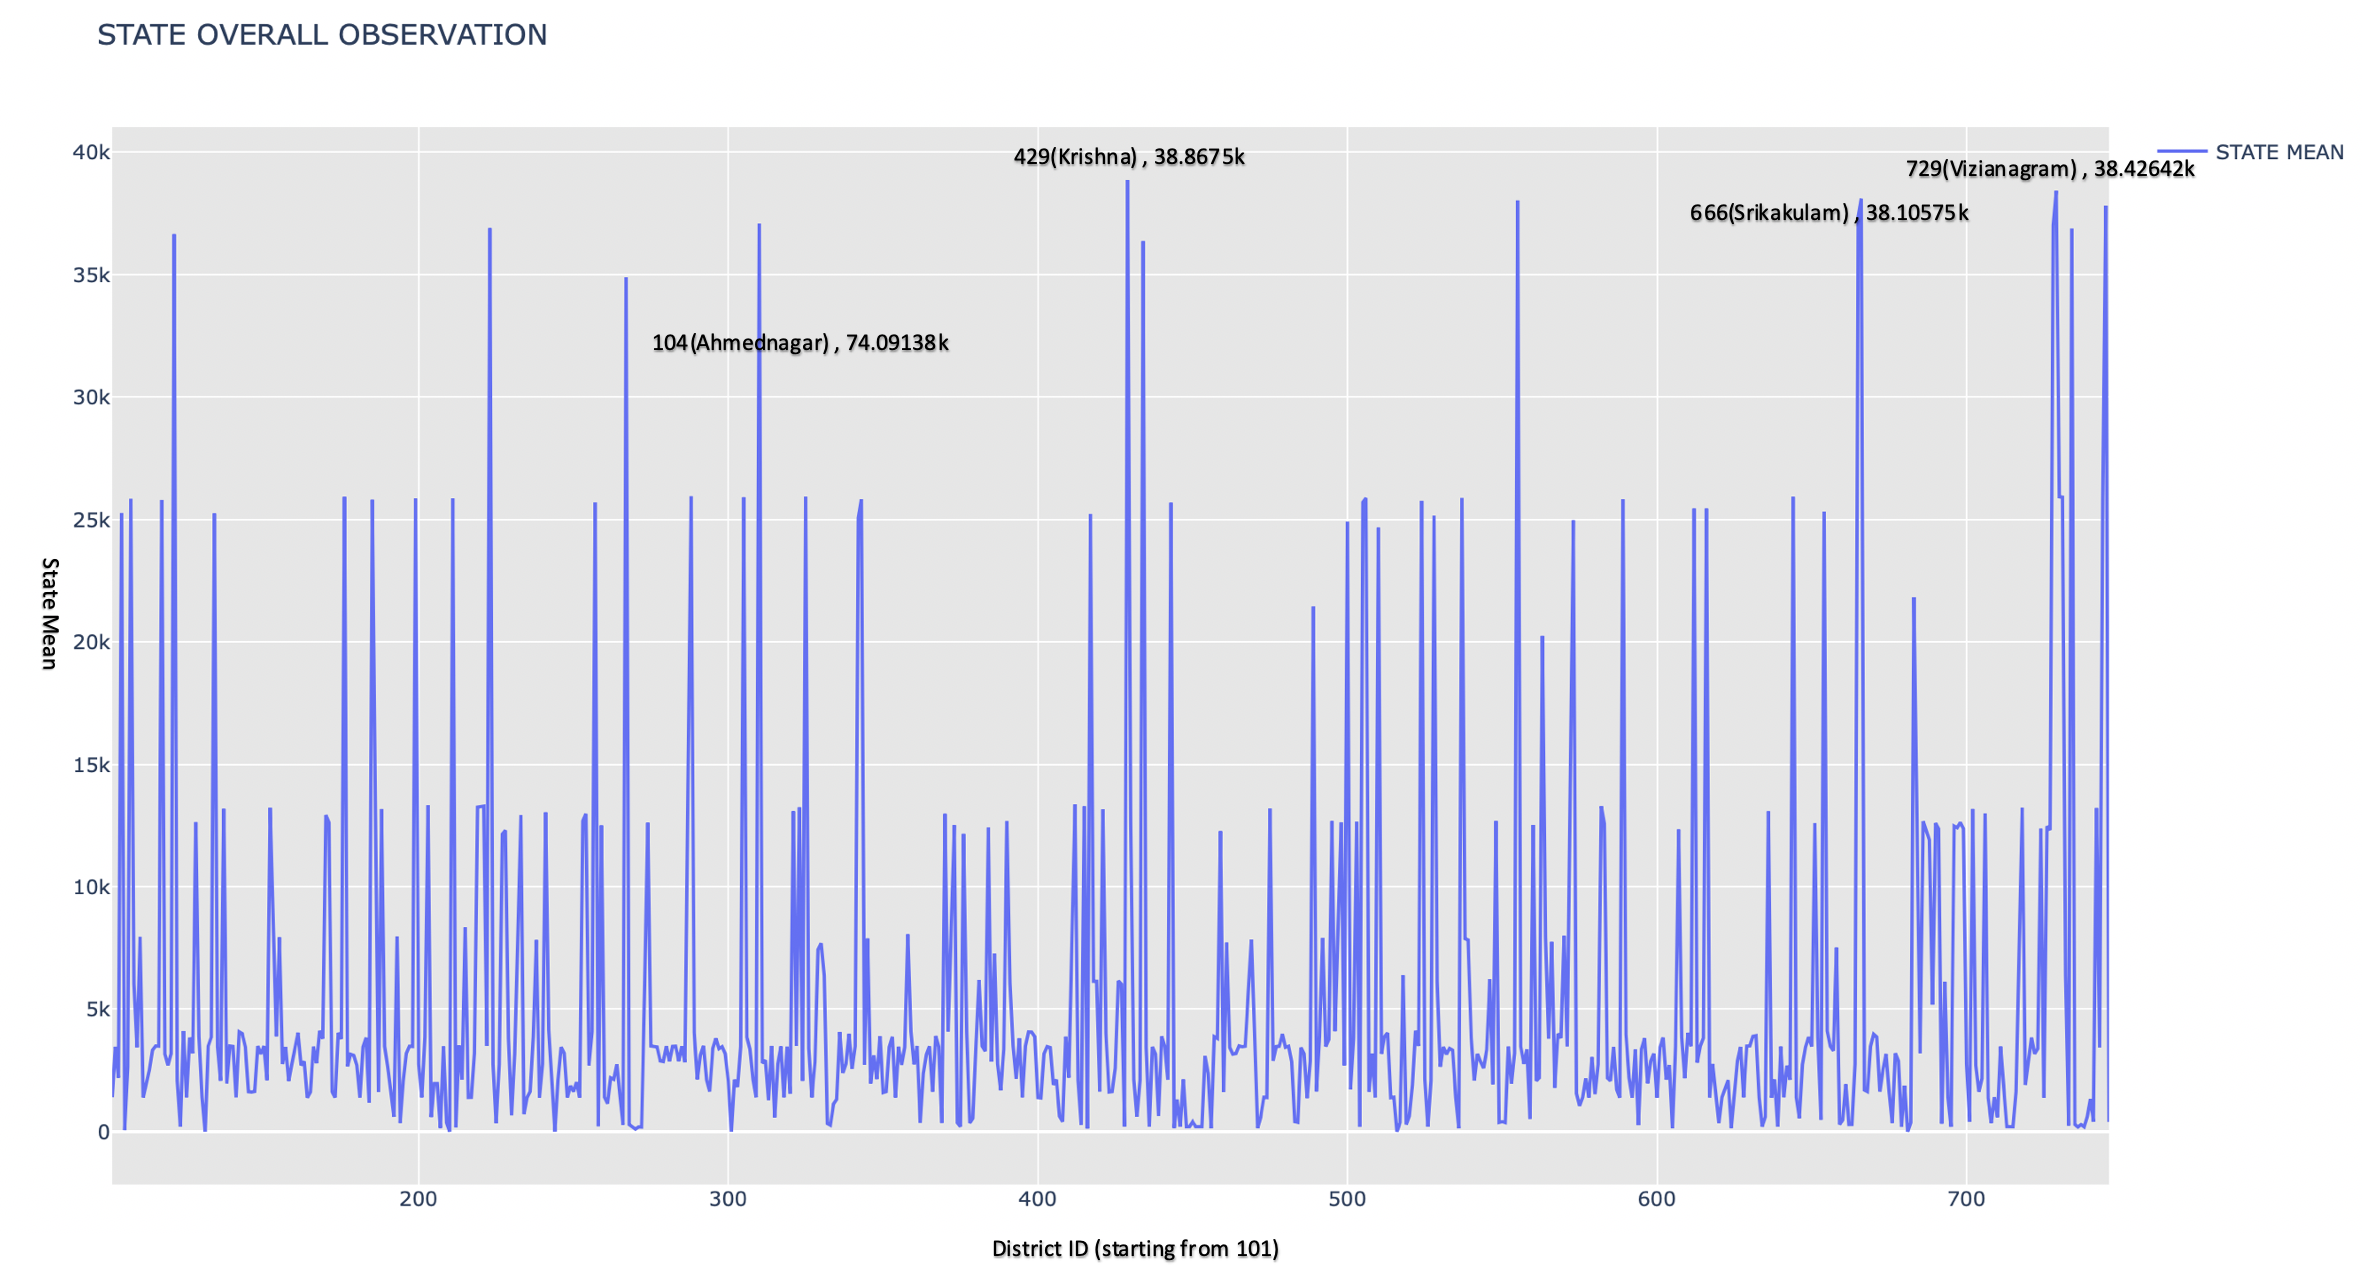
\includegraphics[scale=0.32]{images/State Mean.png}
\centerline{\textbf{Figure 3}} \newline\newline
\justify \textbf{Figure 3} aim to show the impact of COVID-19 on a particular district with respect to the state in which this district lies. The Y-axis shows the average(mean) of the number of cases in the particular state(excluding the district which we are considering) in which a district lies. The X-axis shows for which district we are taking the state mean.
\newline There are many district which shows larger values for state mean, so of these are \textbf{Krishna, Ahmednagar, Srikakulam, Vizianagram} and so on.

\newpage 
\subsection{Neighborhood Z-Score GRAPH}
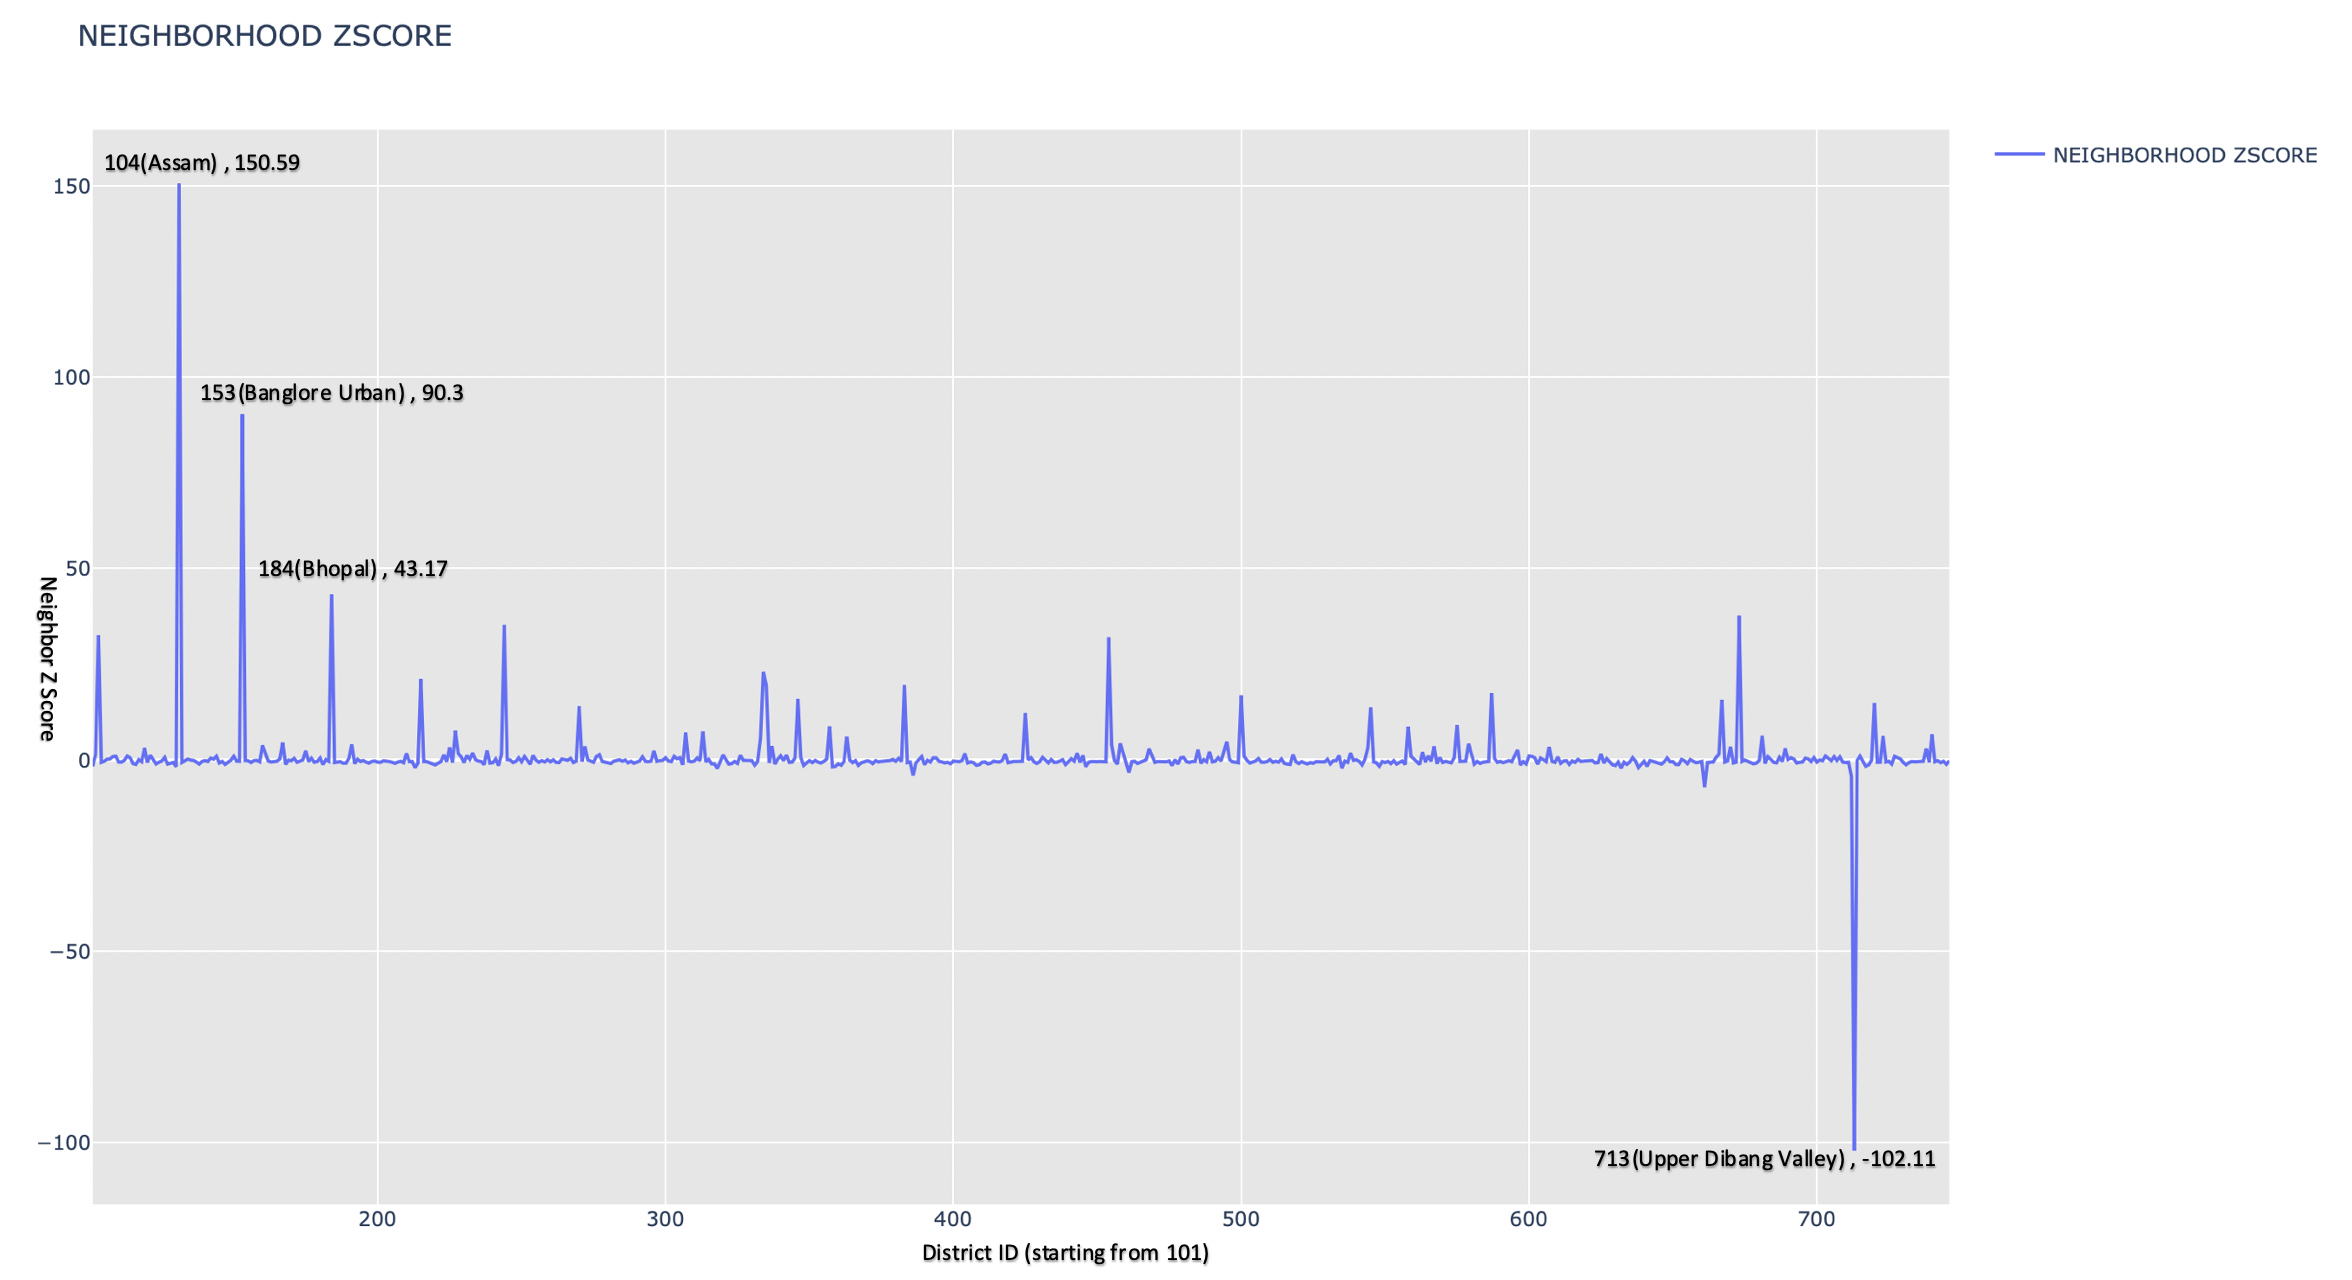
\includegraphics[scale=0.346]{images/Neighbor Z Score.png}
\centerline{\textbf{Figure 4}} \newline\newline
\newline \textbf{ZSCORE = (X - MEAN)/(STANDARD DEVIATION)}, here X represent number of cases in the particular district.
\newline \justify The Y-axis in \textbf{Figure 4} shows the value of Z Score of the neighborhood districts with respect to particular district in X-axis. The value of the Z Score tells you how many standard deviations you are away from the mean. \textbf{Positive Z Score} value of the neighbor districts of the particular district shows that the number of cases in this particular district which we are considering is greater than on average cases of the neighborhood districts. \textbf{Negative Z Score} value of the neighbor districts of the particular district shows that the number of cases in this particular district which we are considering is less than on average cases of the neighborhood districts. 
\newline For example in \textbf{Figure 4} if we consider district \textbf{Bangalore Urban} it has positive Z Score which shows that it has very high number of cases w.r.t. on an average cases of the neighbors of the Bangalore Urban. Similarly if we consider \textbf{Upper Dibang Valley} it has very low number of cases w.r.t. on an average cases of the neighbors io the Upper Dibang Valley.

\newpage 
\subsection{State Z-Score GRAPH}
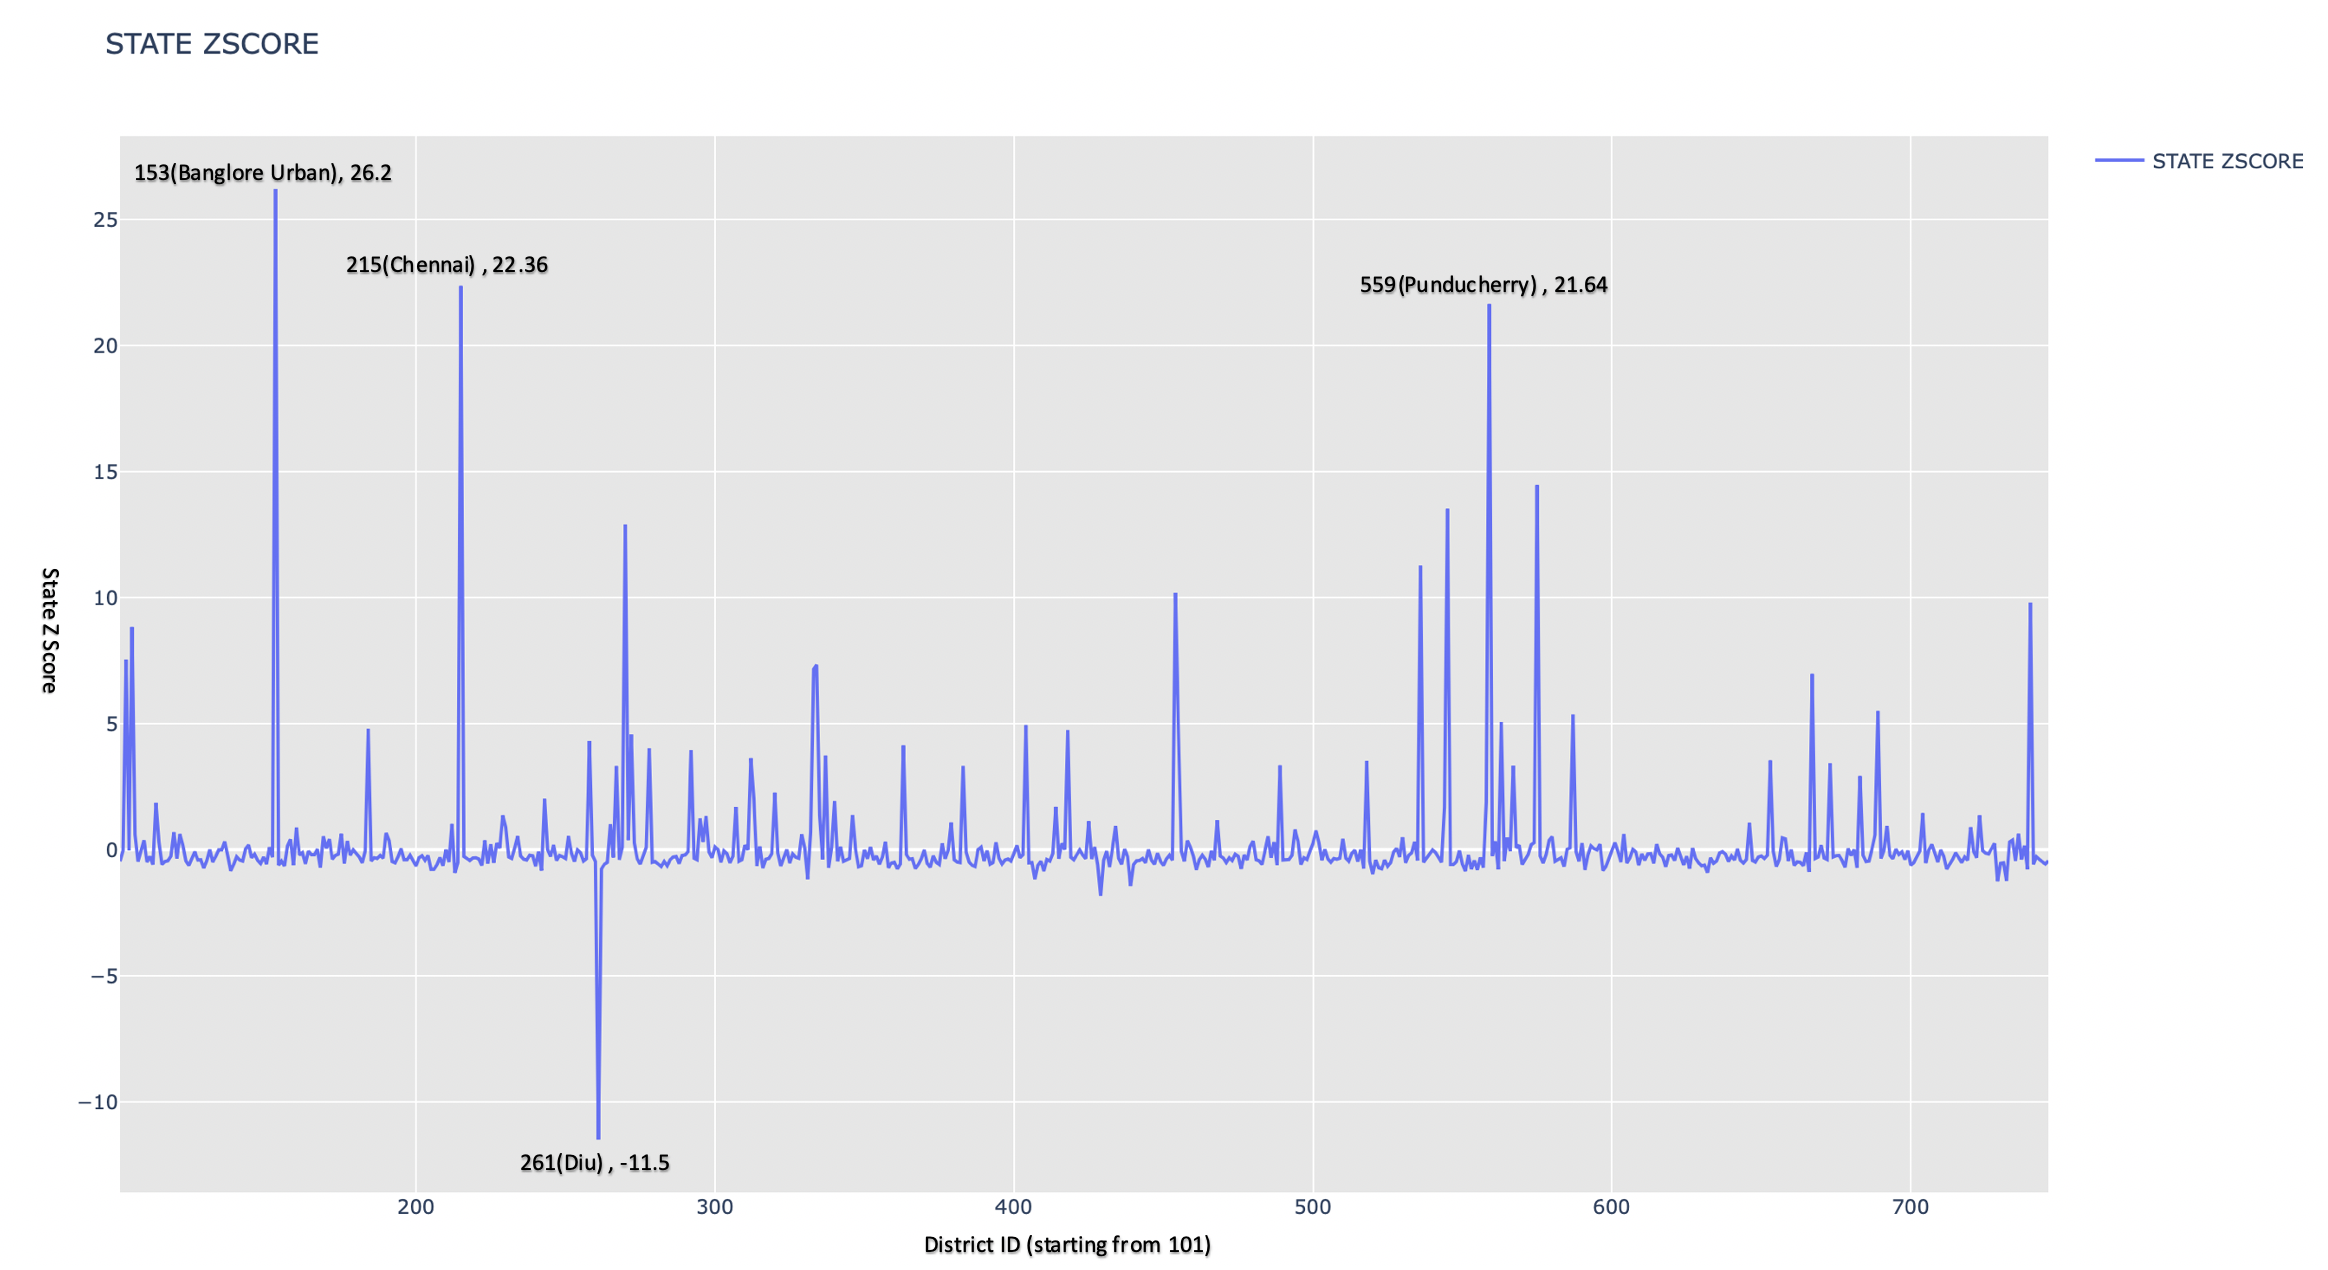
\includegraphics[scale=0.33]{images/State Z Score.png}
\centerline{\textbf{Figure 5}} \newline\newline
\justify The Y-axis in \textbf{Figure 5} shows the value of Z Score of the State in which a particular district lies(X-axis). In this scenario also we are getting both positive and negative value of the Z Score. 
\newline If we consider the district \textbf{Bangalore Urban, Chennai or Pondicherry}, these districts show high value of State Z Score which means that if we consider these districts than the number of cases in this particular district is greater than on average cases in State in which this district lies. This also means than this district contribute large number of cases of COVID-19 to the state in which it lies.
\newline It we consider district \textbf{Diu}, its Z Score is very less means it contribute very less to the total number of cases in particular state.

\newpage
\section{Observations}
\justify 
\textbf{1}. A district is \textbf{Hotspot} with respect to its neighbouring districts or the state in which it lies if \textbf{X \textgreater  (MEAN + STANDARD DEVIATION)}. Here X is the number of cases in the particular district which we are considering. MEAN(average number of cases) and STANDARD DEVIATION(amount of variation or dispersion of a number of cases) in either neighbourhood districts or State in which this district lies. \newline If we consider a district say DISTRICT1 and if it satisfies the formula that means the number of cases in DISTRICT1 is too high that it crosses the range of average cases along with the dispersion of COVID-19 cases. \textit{For a State/Neighbor, a district is considered as Hotspot if it contribute very large number of COVID-19 cases to the overall cases in State/Neighbor.}  \newline 
\textbf{2}. A district is \textbf{Coldspot} with respect to its neighbouring districts or the state in which it lies if \textbf{X \textless  (MEAN - STANDARD DEVIATION)}. Here X is the number of cases in the particular district which we are considering. MEAN(average number of cases) and STANDARD DEVIATION(amount of variation or dispersion of a number of cases) in either neighbourhood districts or State in which this district lies. \textit{For a State/Neighbor, a district is considered as Coldspot if it contribute very less number of COVID-19 cases to the overall cases in State/Neighbor.}  \newline 

\section{Prediction}
\justify 1. The districts that can be Hotspot or Coldspot in the future days based on its neighbourhood mean and standard devation. \newline
2. The number of cases in a particular district may increase if the Z-score of its neighbourhood or state is positive. \newline
3. If Z Score of any district is lower than 0 than there may be chance that if can largely affect its neighbourhood districts or state in which it lies. \newline
4. If a district become Coldspot/Hotspot than there may be chances that the neighbourhood districts or the state in which it lies has MORE/LESS number of cases on average with respect to this district. \newline
5. Before visiting any district one can find out whether this district is Hotspot or Coldspot with respect to its neighborhood or state than plans accordingly.

\newpage
\section{Precautions}
\justify To prevent the spread of COVID-19: \newline
1.Clean your hands often. Use soap and water, or an alcohol-based hand rub. \newline
2. Maintain a safe distance from anyone who is coughing or sneezing. \newline
3. Wear a mask when physical distancing is not possible. \newline
4. Don’t touch your eyes, nose or mouth. \newline
5. Cover your nose and mouth with your bent elbow or a tissue when you cough or sneeze. \newline
6. Stay home if you feel unwell. \newline
7. If you have a fever, cough and difficulty breathing, seek medical attention. \newline

\section{Conclusions}
\justify The coronavirus disease continues to spread across the world following a trajectory that is difficult to predict. After considering the above statistics of COVID-19 cases through Graphs one can choose either to visit that district or not. If they visit how much awareness he/she need to maintain. What precautions he/she need to take when he/she visit there.
\newline \centerline{\textbf{Special Thanks to all the Doctors.}}
\section{GitHub Code link}
\href{https://github.com/kuldeeps5/Data-Mining-Assignment-1}{https://github.com/kuldeeps5/Data-Mining-Assignment-1}
\section{References}
\href{https://api.covid19india.org/documentation/csv/}{https://api.covid19india.org/documentation/csv/} \newline
\href{https://www.who.int/emergencies/diseases/novel-coronavirus-2019/advice-for-public}{https://www.who.int/}
\end{document}